\documentclass[tikz,border=10pt]{standalone}
\usepackage{pgfplots}
\pgfplotsset{compat=1.18}
\usepackage{amsmath}
\usepackage{amssymb}
\definecolor{mantis}{RGB}{0, 105, 62}
\begin{document}
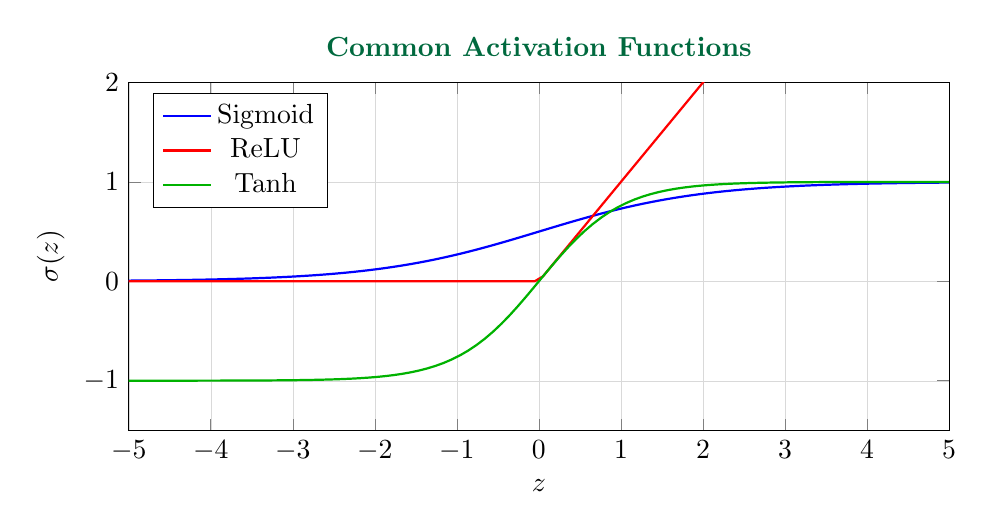
\begin{tikzpicture}
\begin{axis}[
    width=12cm,
    height=6cm,
    xlabel={$z$},
    ylabel={$\sigma(z)$},
    xmin=-5, xmax=5,
    ymin=-1.5, ymax=2,
    legend pos=north west,
    title={\textbf{Common Activation Functions}},
    title style={font=\bfseries\color{mantis}},
    grid=both,
    grid style={line width=.1pt, draw=gray!30},
]
% Sigmoid
\addplot[domain=-5:5, samples=100, color=blue, thick] {1/(1+exp(-x))};
% ReLU
\addplot[domain=-5:5, samples=100, color=red, thick] {max(0,x)};
% Tanh
\addplot[domain=-5:5, samples=100, color=green!70!black, thick] {tanh(x)};
\legend{Sigmoid, ReLU, Tanh}
\end{axis}
\end{tikzpicture}
\end{document}
